
	El algoritmo de Kalman se basa en poder estimar el vector de estados a partir de la dinámica del sistema y las mediciones. Para la definición del algoritmo se utilizará la siguiente notación. Se llamará:
	
	\begin{equation*}
		\vect{x}_{k/k - 1}
	\end{equation*}
	a la mejor estimación del vector de estados utilizando información hasta el instante $k - 1$. Es decir se trata de una predicción. Se llamará a la matriz de covarianza del error de dicha estimacion:
	
	\begin{equation*}
		P_{k/k - 1}
	\end{equation*}
	
	Por otro lado se llamará a:
	
	\begin{equation*}
		\vect{x}_{k/k}
	\end{equation*}
	a la mejor estimación del vector de estados utilizando información hasta el instante $k$. Dicha estimación será el resultado final del algoritmo y la matriz de covarianza del error del mismo será:
	
	\begin{equation*}
		P_{k/k - 1}
	\end{equation*}

	Cabe aclarar que cuando se habla del mejor estimador, se referiere a aquel que minimiza el error cuadrático medio.\\
	
		\subsection{Algoritmo de Kalman}
			\paragraph{Inicialización}
				Es la etapa en la cual se define el estado inicial de la estimación. Para poder inicializar el algoritmo se necesita una estadística del estado inicial del sistema:
				
				\begin{equation*}
					\vect{x}_{0/0} \leftarrow E\left[\vect{x}_{0}\right]
				\end{equation*}
				
				\begin{equation*}
					P_{0/0} \leftarrow \text{cov}\left[\vect{x}_{0}\right]
				\end{equation*}
			\paragraph{Predicción}
				Es la etapa en la cual se realiza una predicción del futuro estado del sistema utilizando el modelo en el espacio de estados:
				
				\begin{equation*}
					\vect{x}_{k/k - 1} \leftarrow A_{d_{k - 1}} \; \vect{x}_{k - 1/k - 1}
				\end{equation*}
				
				\begin{equation*}
					P_{k/k - 1} \leftarrow A_{d_{k - 1}}\; P_{k - 1 / k - 1}\; A_{d_{k - 1}}^{*} + B_{d_{k - 1}}\; Q_{k - 1}\; B_{d_{k - 1}}^{*}
				\end{equation*}
			\paragraph{Corrección}
				Es la etapa en la cual se corrige la predicción con el valor de la medición. Para ello se necesita calcular la matriz de ganancia de Kalman $K_{k}$:
				
				\begin{equation*}
					K_{k} \leftarrow P_{k / k - 1}\; C_{d_{k}}^{*}\; (C_{d_{k}}\; P_{k/k - 1}\; C_{d_{k}}^{*}\; + R_{k})^{-1}
				\end{equation*}
				
				Luego se corrige:
				
				\begin{equation*}
					\vect{x}_{k/k} \leftarrow \vect{x}_{k/k - 1} + K_{k}\; (y_{k} - C_{d_{k}}\; \vect{x}_{k/k - 1})
				\end{equation*}
				
				\begin{equation*}
					P_{k/k} \leftarrow (I - K_{k}\; C_{d_{k}})\; P_{k/k - 1}
				\end{equation*}
					
			\paragraph{Actualización}
				Es la etapa del algoritmo en la que se pasa al siguiente instante $k$.
				
				\begin{equation*}
					\vect{x}_{k - 1/k - 1} \leftarrow \vect{x}_{k/k}
				\end{equation*}
				
				\begin{equation*}
					P_{k - 1/k - 1} \leftarrow P_{k/k}
				\end{equation*}


	\subsection{Resultados}
		\subsubsection{Medición De Posición}
			En la Figura \ref{fig:ej2a} se observan los resultados de la estimación basada en mediciones de posición. Puede verse que la estimación se desvía menos del valor real que las mediciones.

		\begin{figure}[H]
			\centering
			%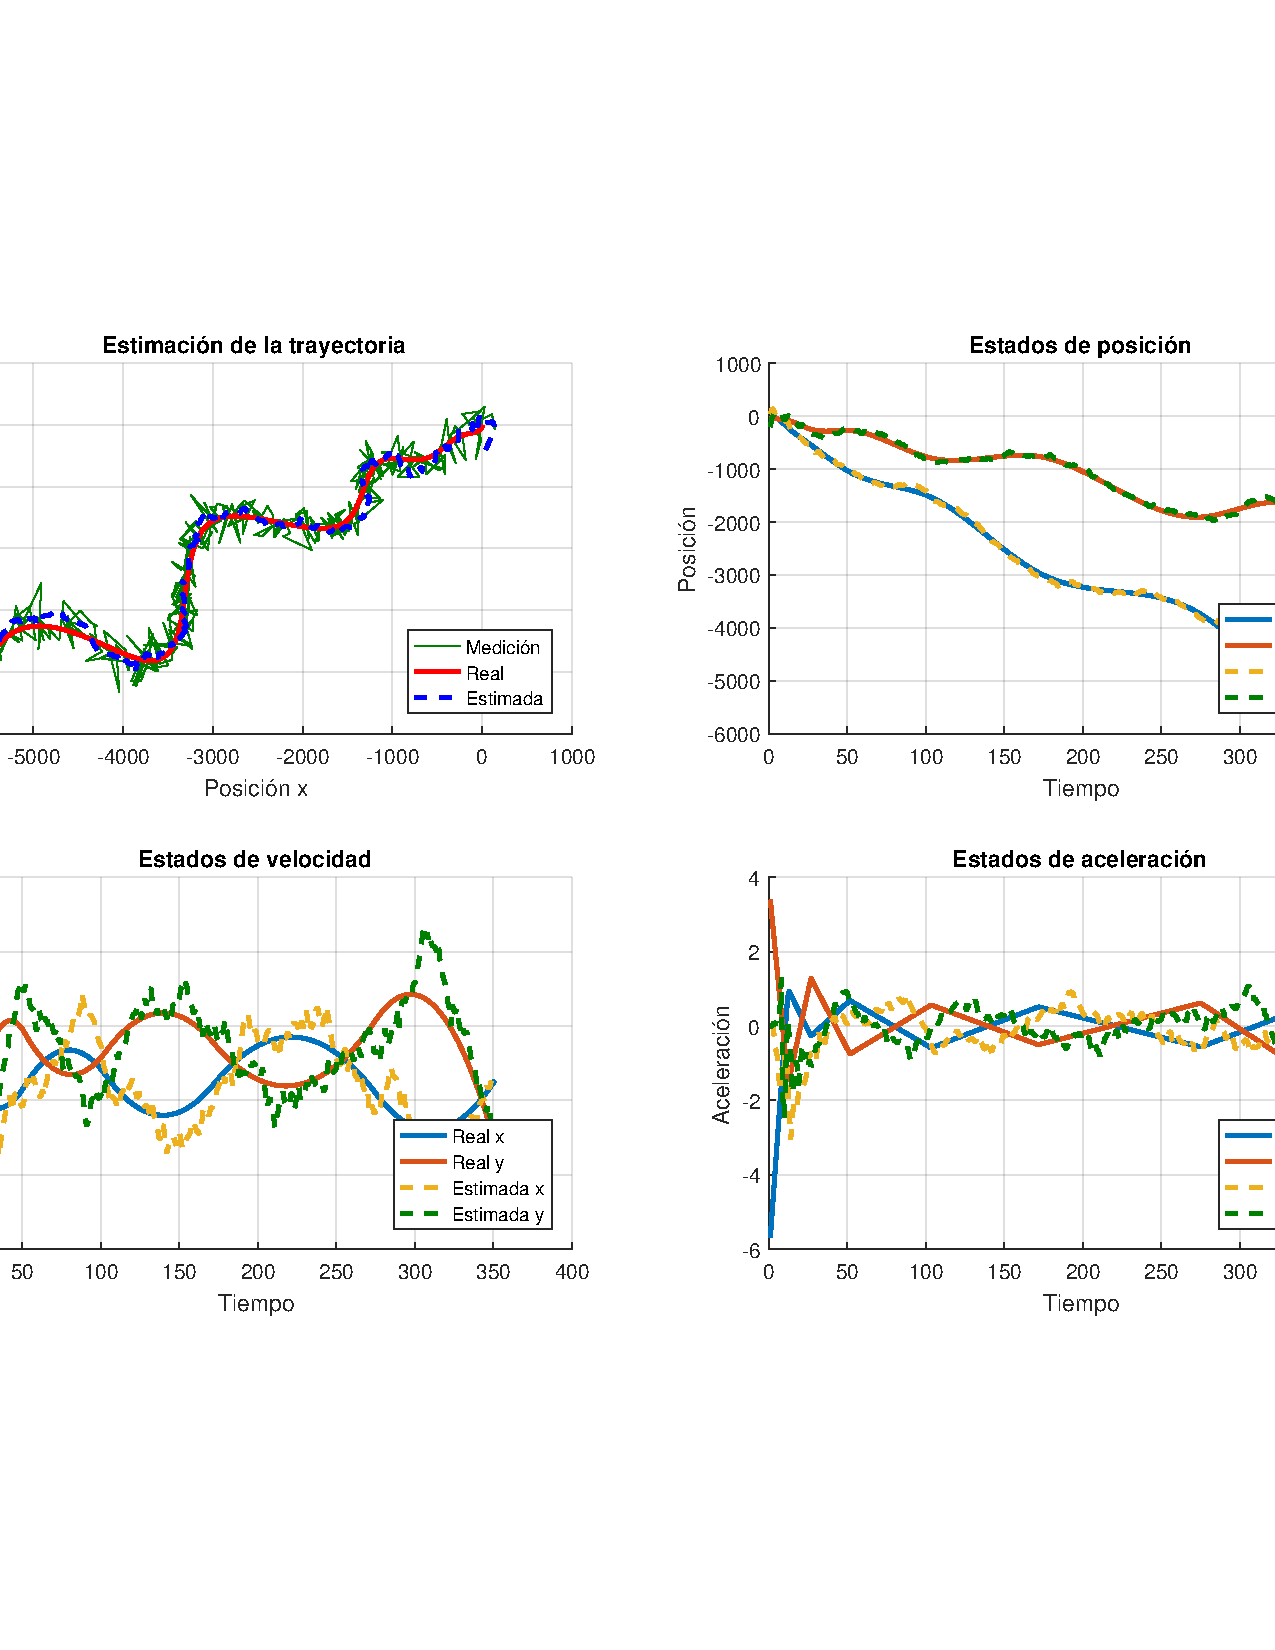
\includegraphics[width=1.0\textwidth,keepaspectratio]{Figuras/graf_ej2a.pdf}
			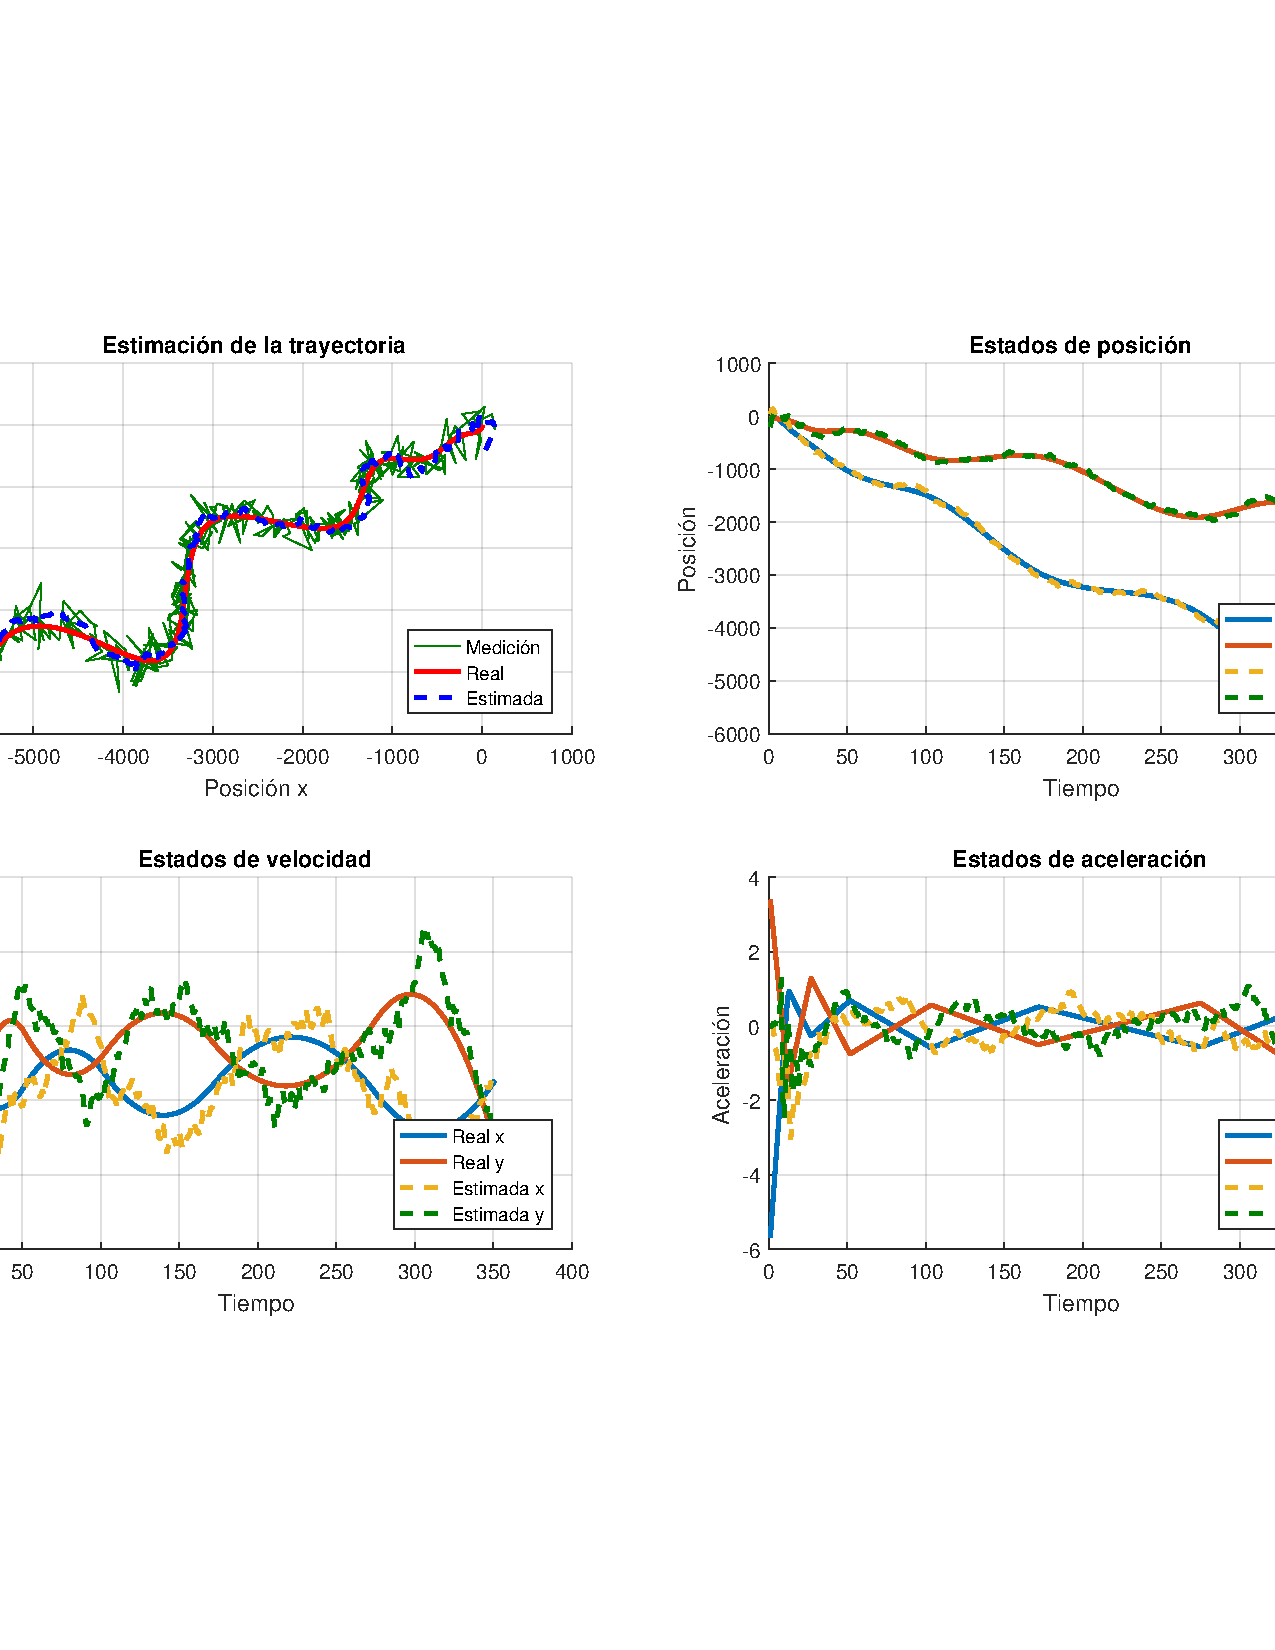
\includegraphics[scale=0.5,trim={6,5cm 0 0 0}]{Figuras/graf_ej2a.pdf}
			\caption{Medición De Posición}
			\label{fig:ej2a}
		\end{figure}
		
		En la Figura \ref{fig:ej2a_innov} se ve la correlación de las innovaciones, donde se observa que se aproximan a un proceso blanco.
		
		\begin{figure}[H]
			\centering
			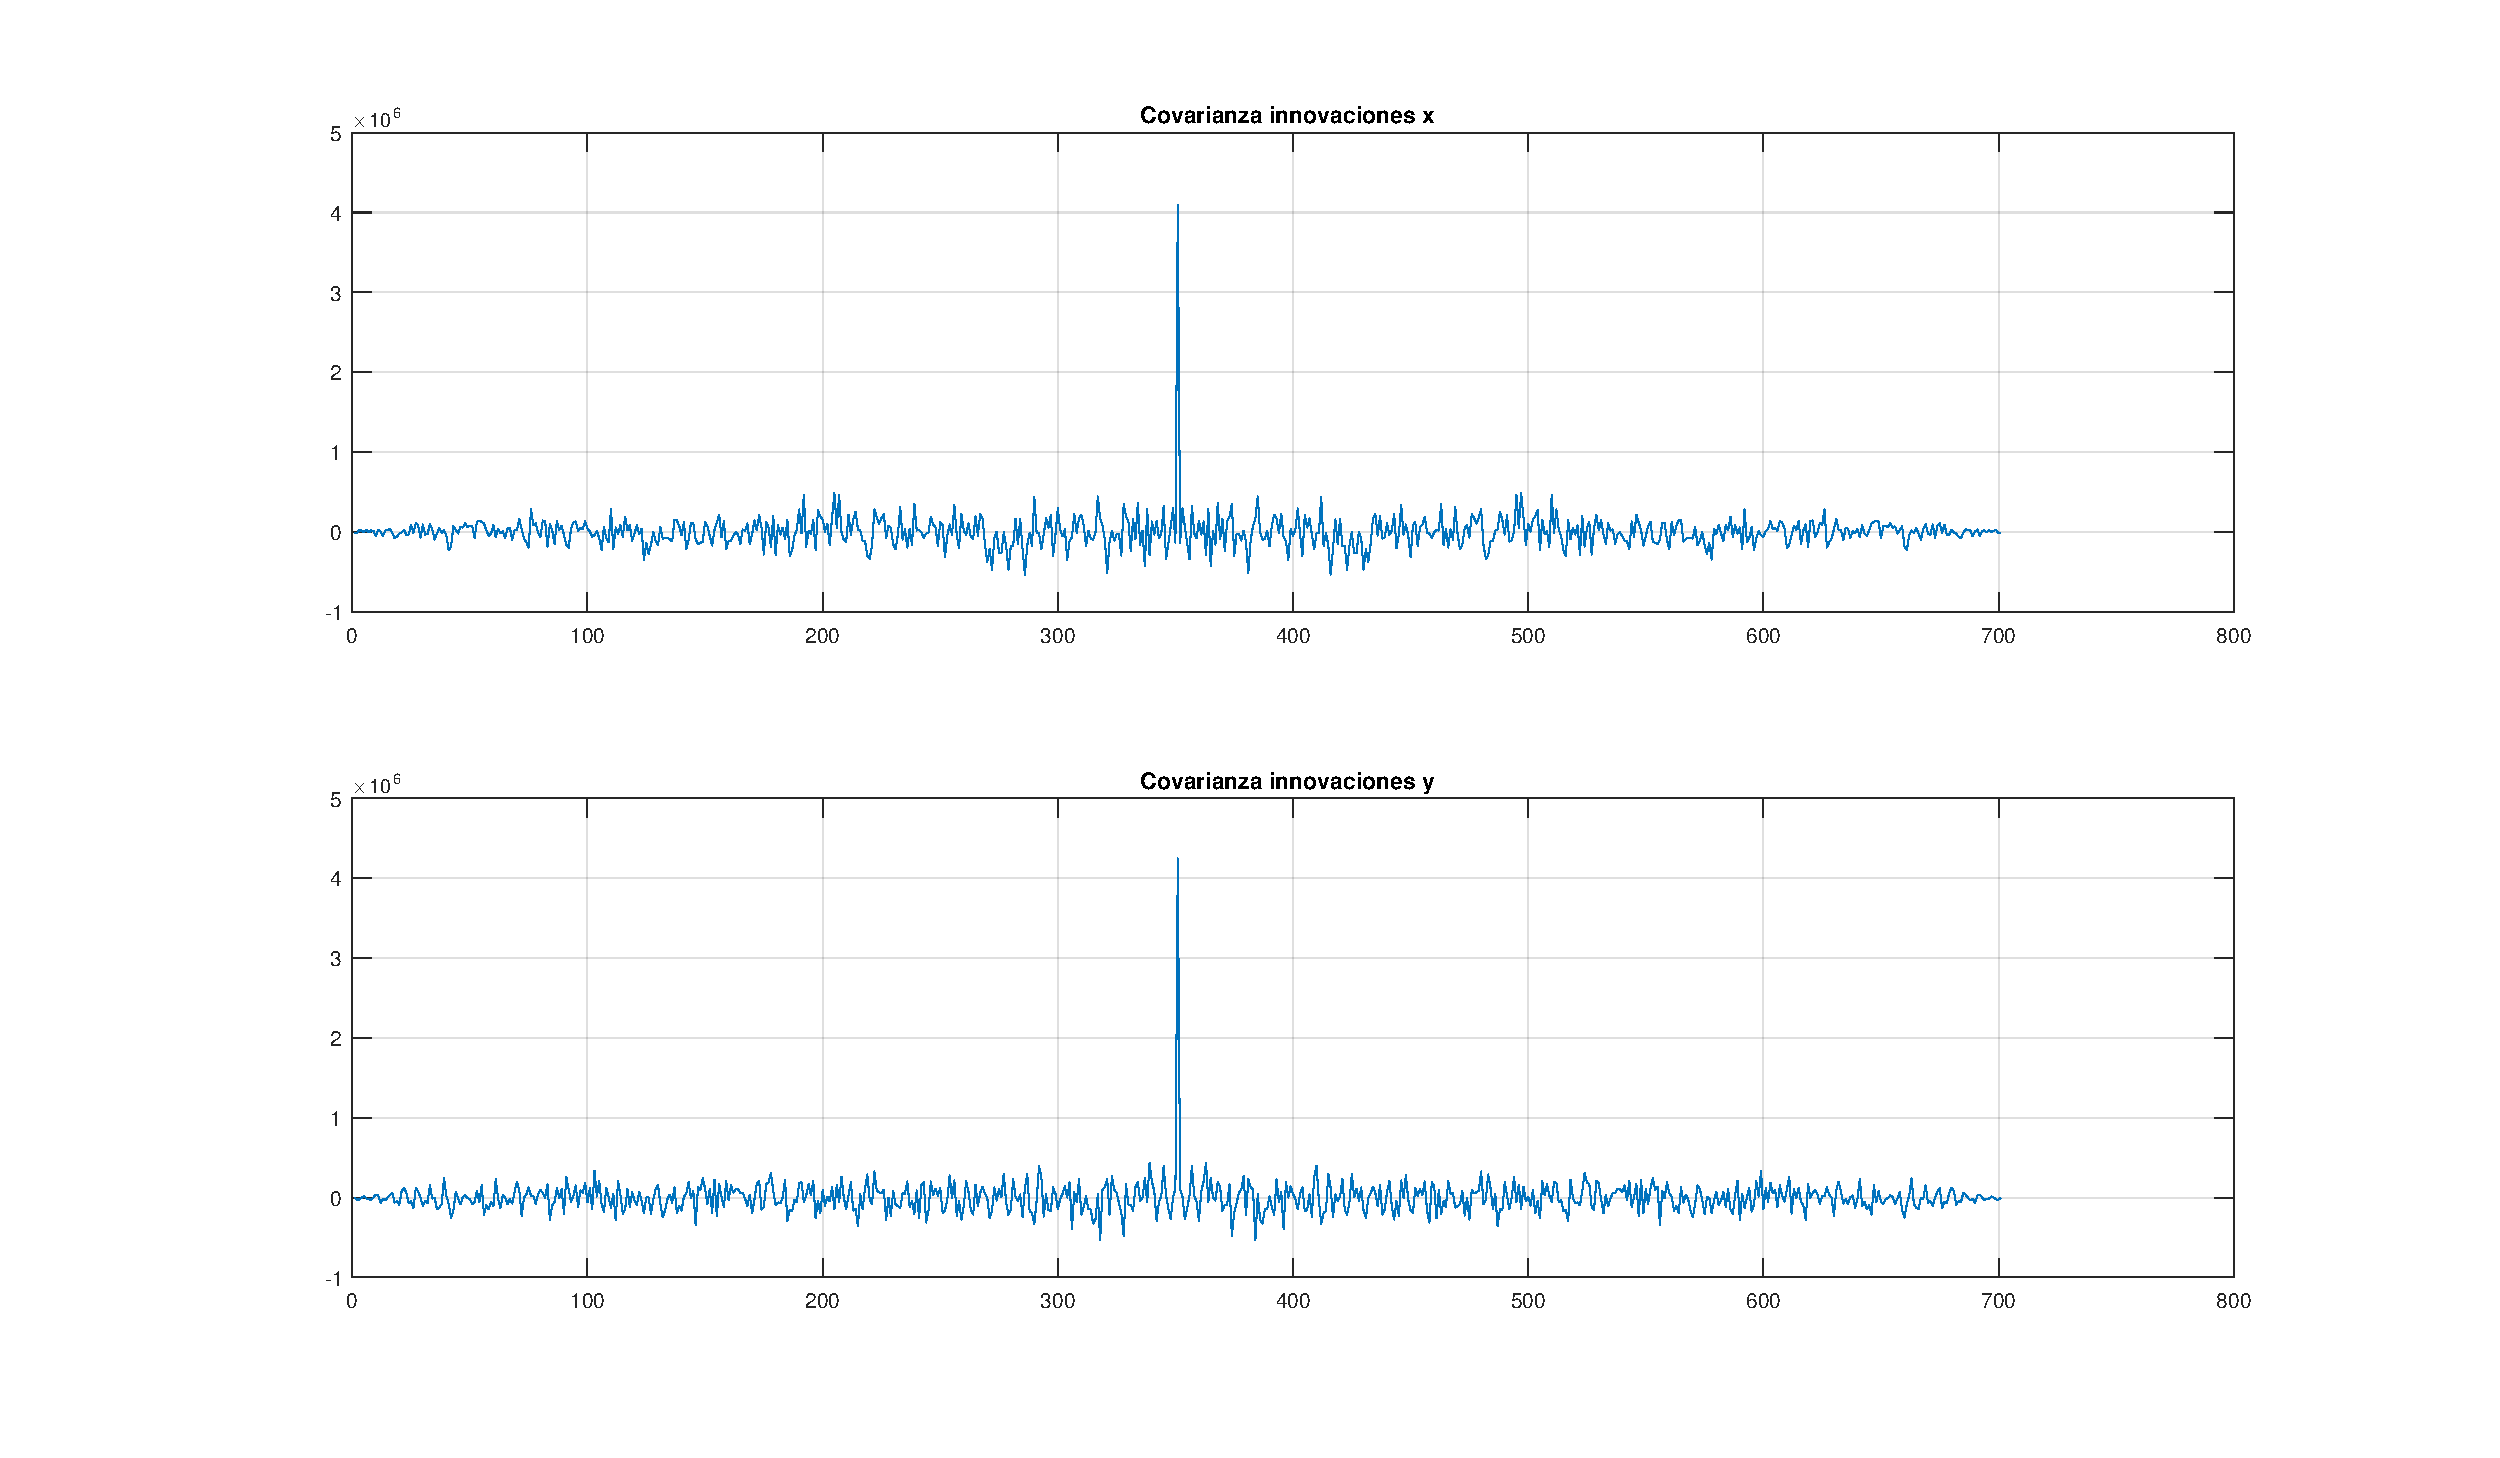
\includegraphics[width=1.0\textwidth,keepaspectratio]{Figuras/covinn_ej2a.pdf}
			\caption{Medición De Posición - Innovaciones}
			\label{fig:ej2a_innov}
		\end{figure}
		
		\subsubsection{Medición De Velocidad}
		
		En la Figura \ref{fig:ej2b} se observa los resultados de la estimación basada en mediciones de velocidad. Puede verse que hay una desviación de la estimación respecto de la trayectoria real.
		
		\begin{figure}[H]
			\centering
			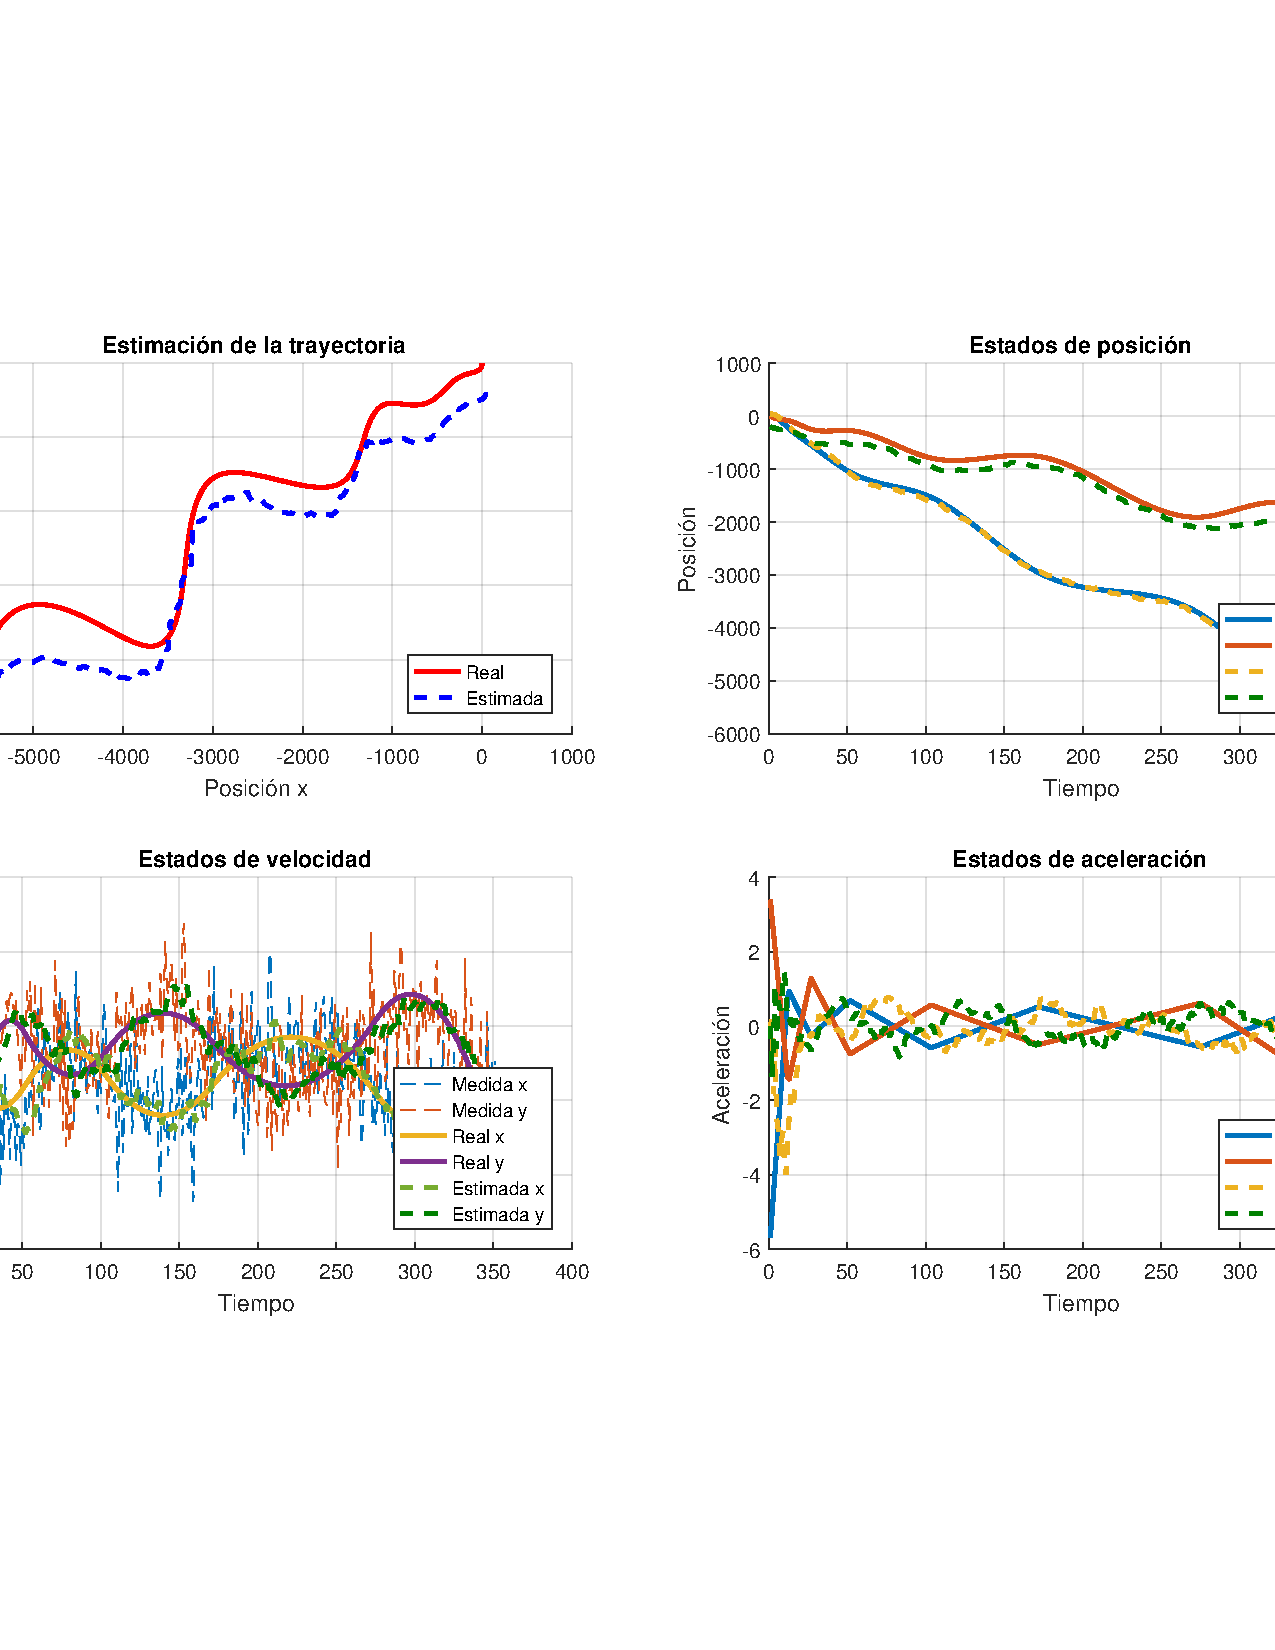
\includegraphics[scale=0.5,trim={6,5cm 0 0 0}]{Figuras/graf_ej2b.pdf}
			\caption{Medición De Velocidad}
			\label{fig:ej2b}
		\end{figure}
		
		En la Figura \ref{fig:ej2b_innov} se ve la correlación de las innovaciones, donde se observa que se aproximan a un proceso blanco.
		
		\begin{figure}[H]
			\centering
			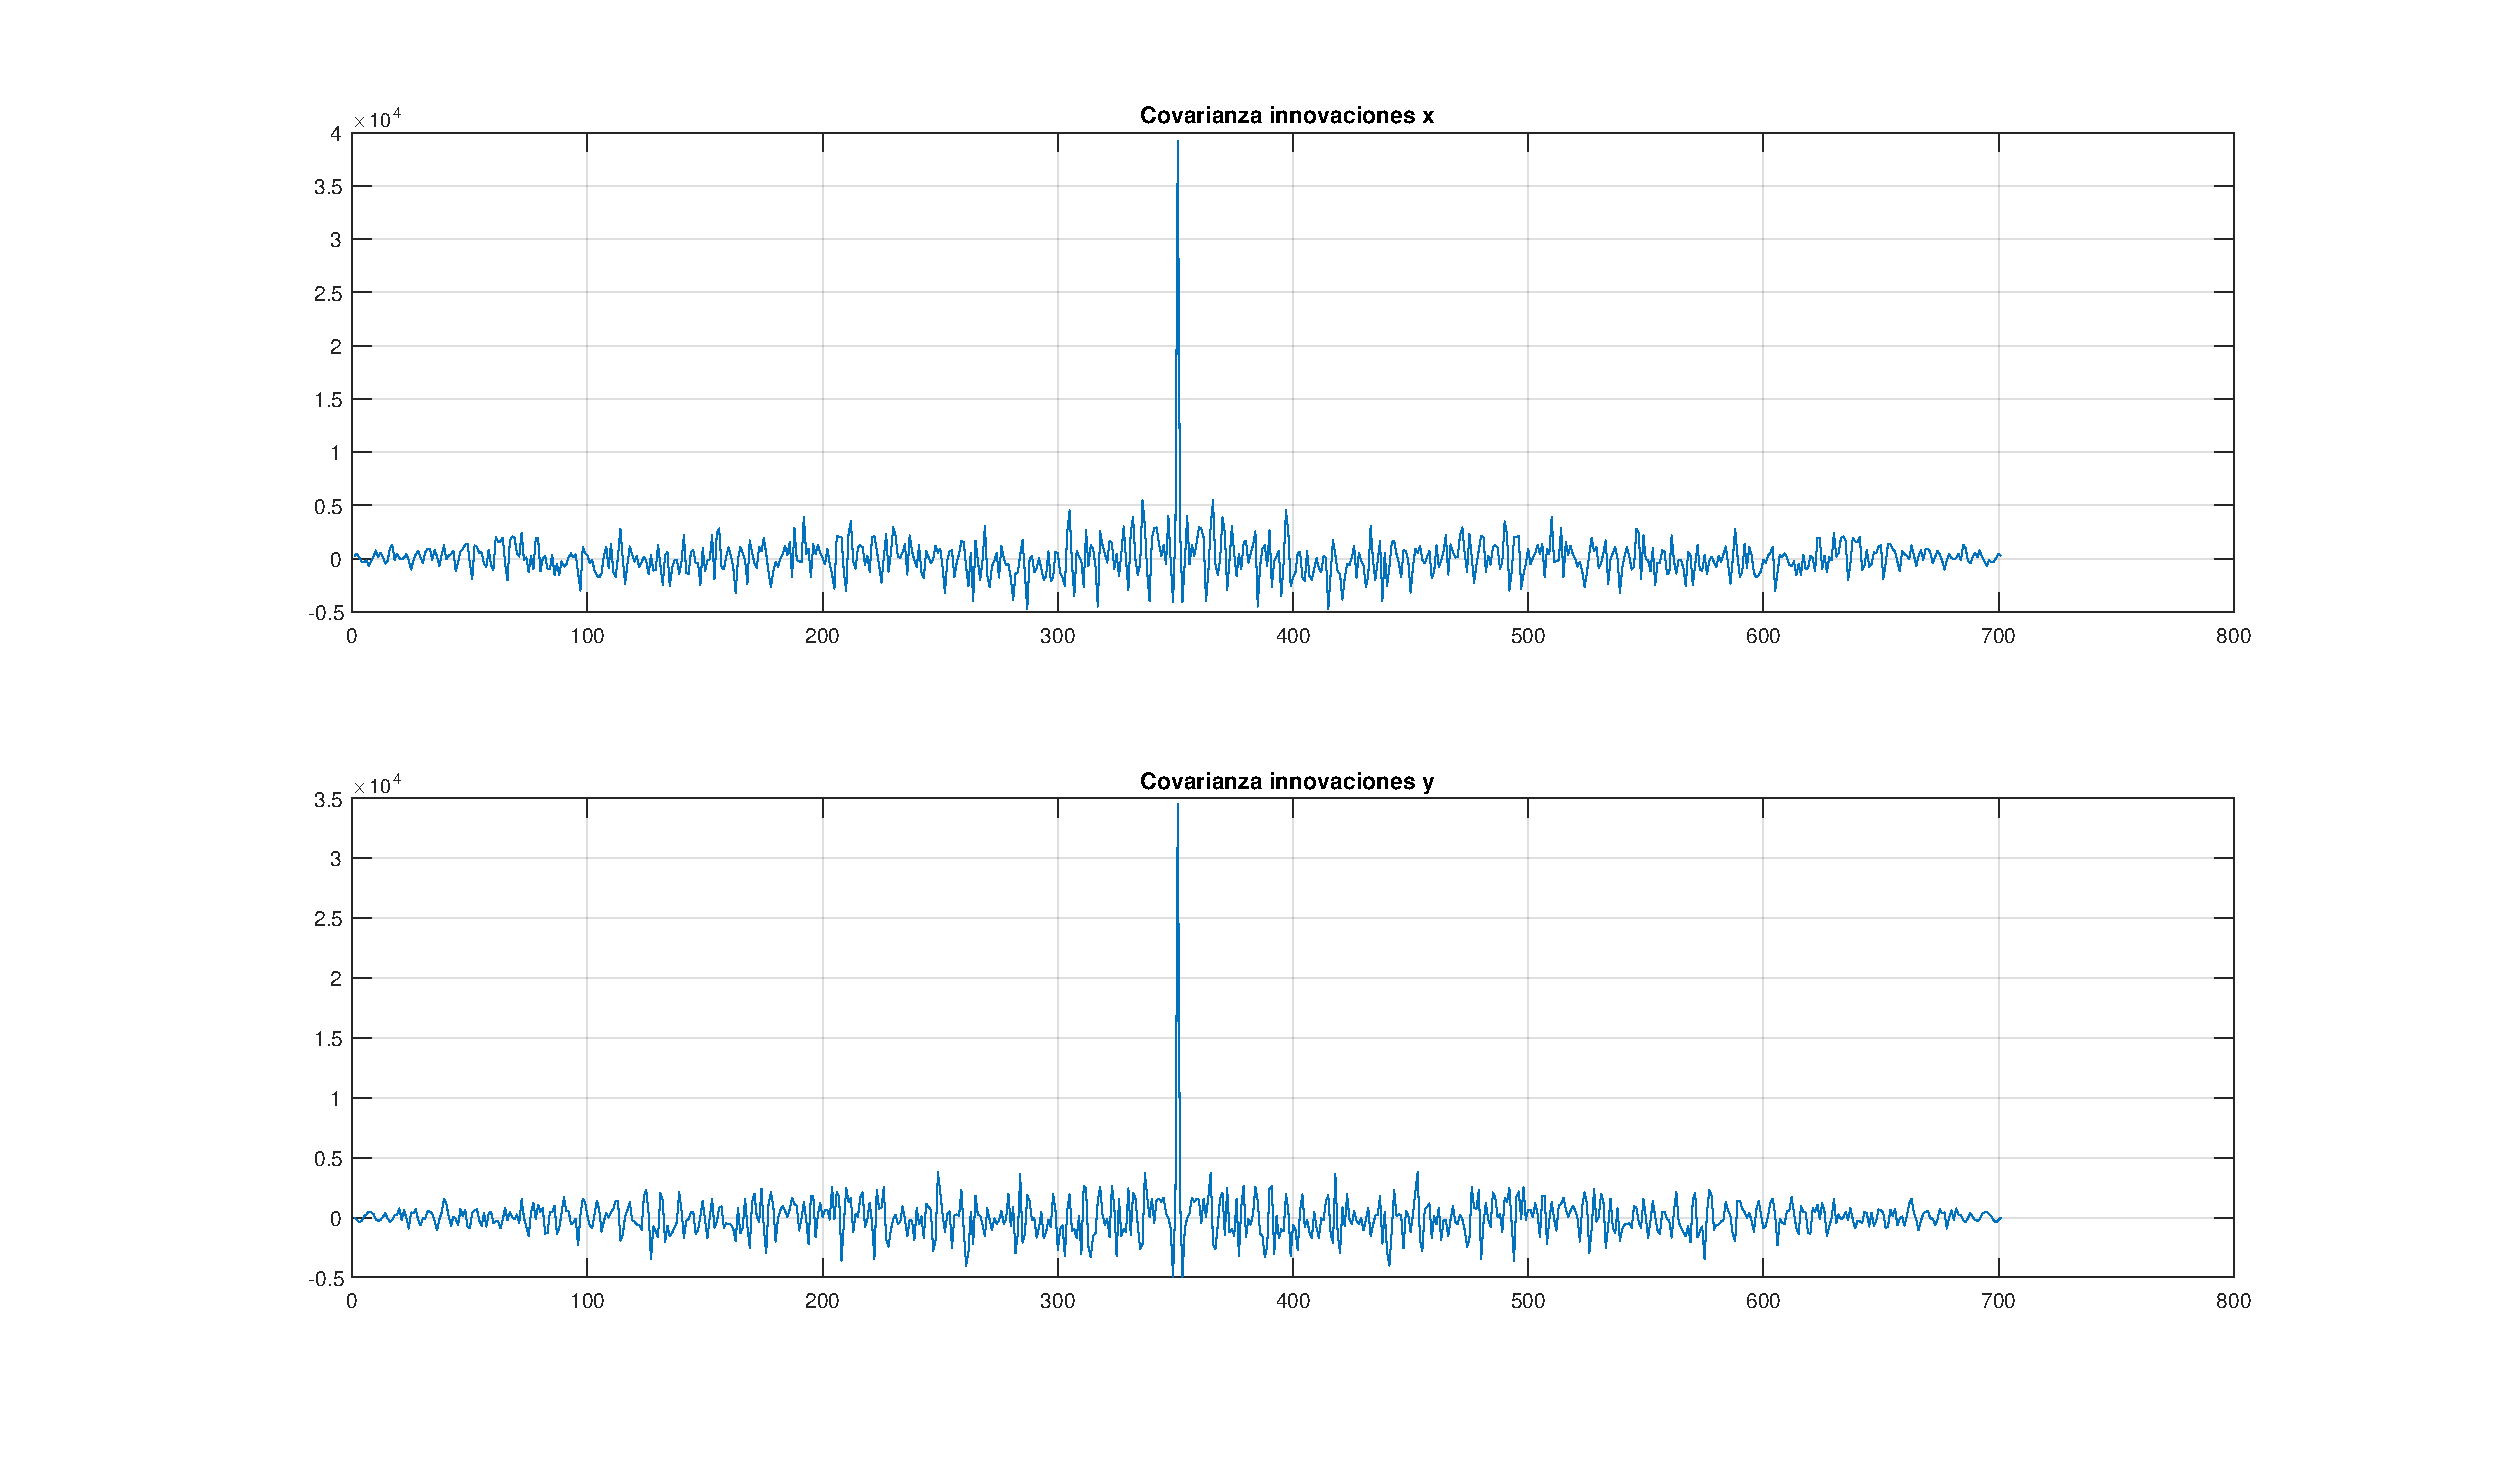
\includegraphics[width=1.0\textwidth,keepaspectratio]{Figuras/covinn_ej2b.pdf} \caption{Medición De Velocidad - Innovaciones} \label{fig:ej2b_innov}
		\end{figure}
			
		\subsubsection{Medición De Aceleración}
		
		En la Figura \ref{fig:ej2c} se observa los resultados de la estimación basada en mediciones de aceleración. Puede verse que la trayectoria estimada nunca sigue a la real.
		
		\begin{figure}[H]
			\centering
			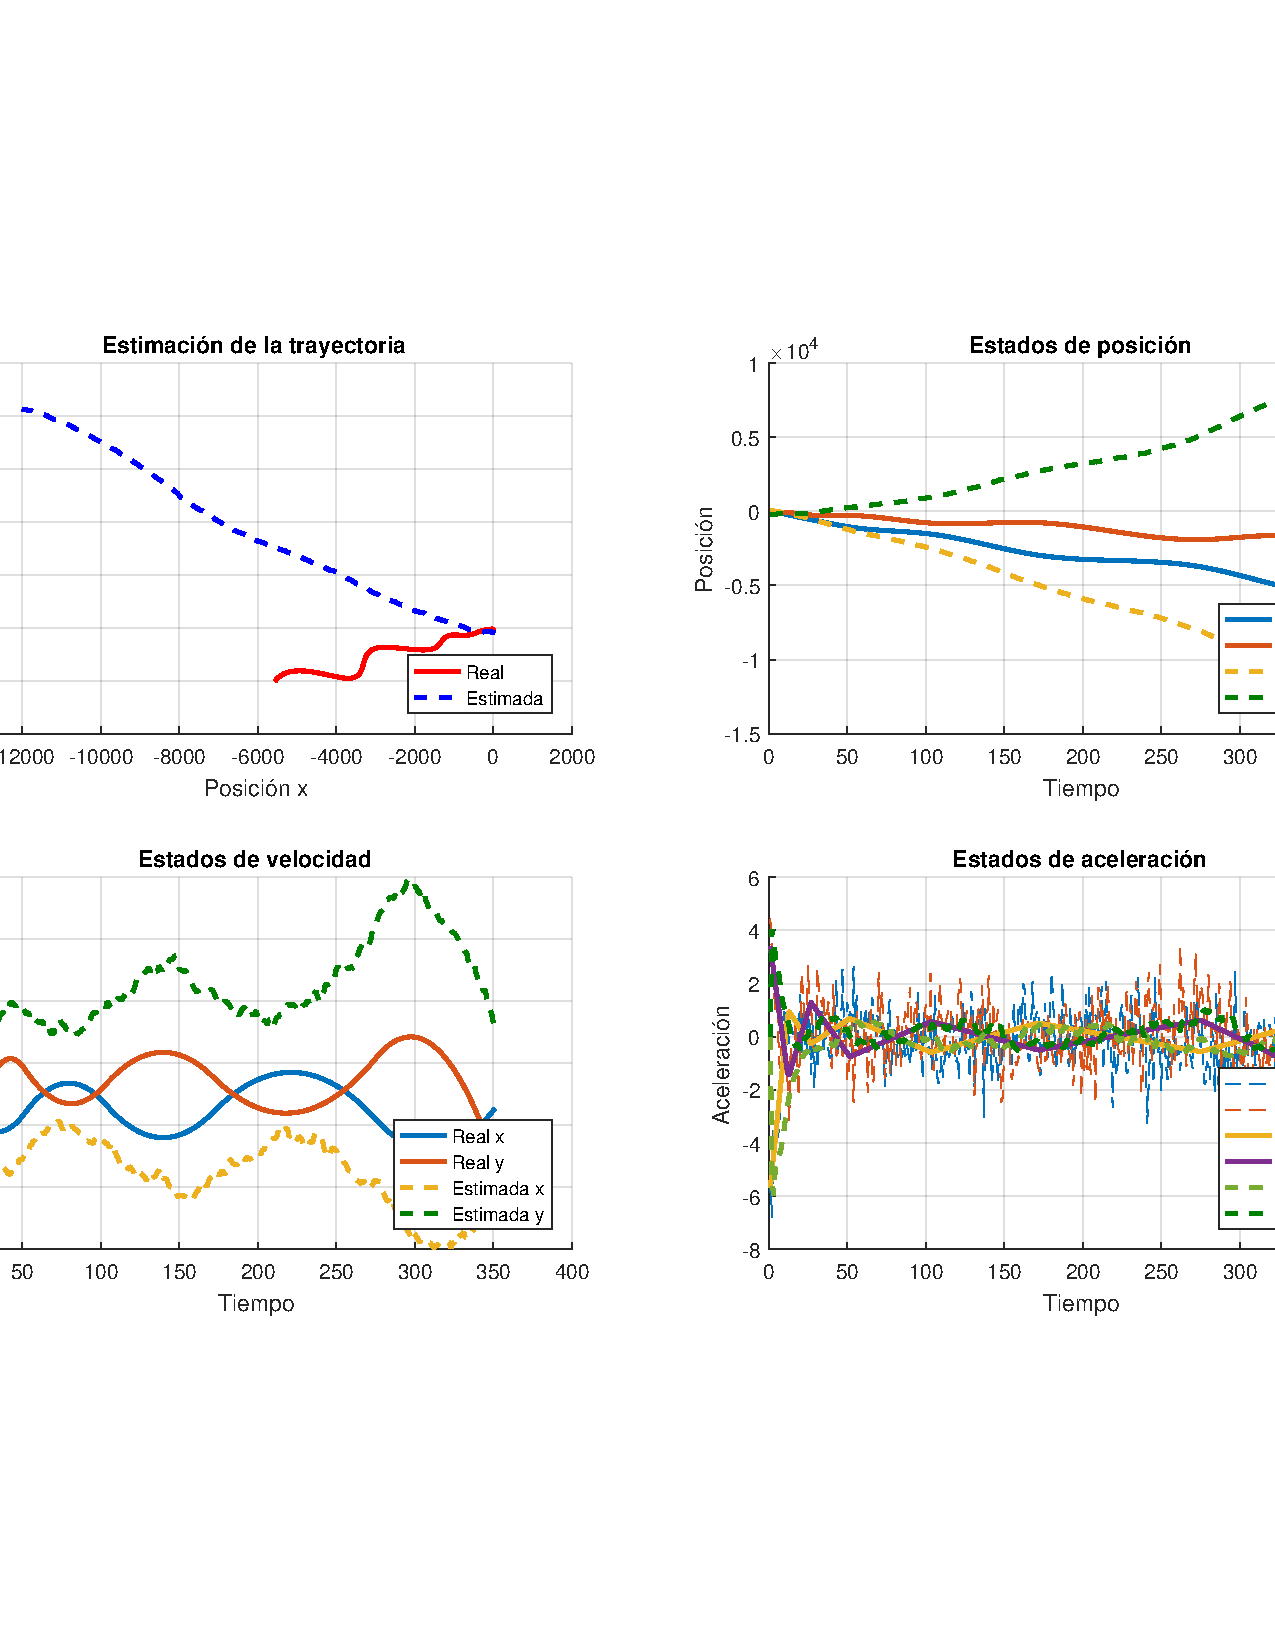
\includegraphics[scale=0.5,trim={6,5cm 0 0 0}]{Figuras/graf_ej2c.pdf}
			\caption{Medición De Aceleración}
			\label{fig:ej2c}
		\end{figure}
		
		En la Figura \ref{fig:ej2c_innov} se ve la correlación de las innovaciones, donde se observa que se aproximan a un proceso blanco.
		
		\begin{figure}[H]
			\centering
			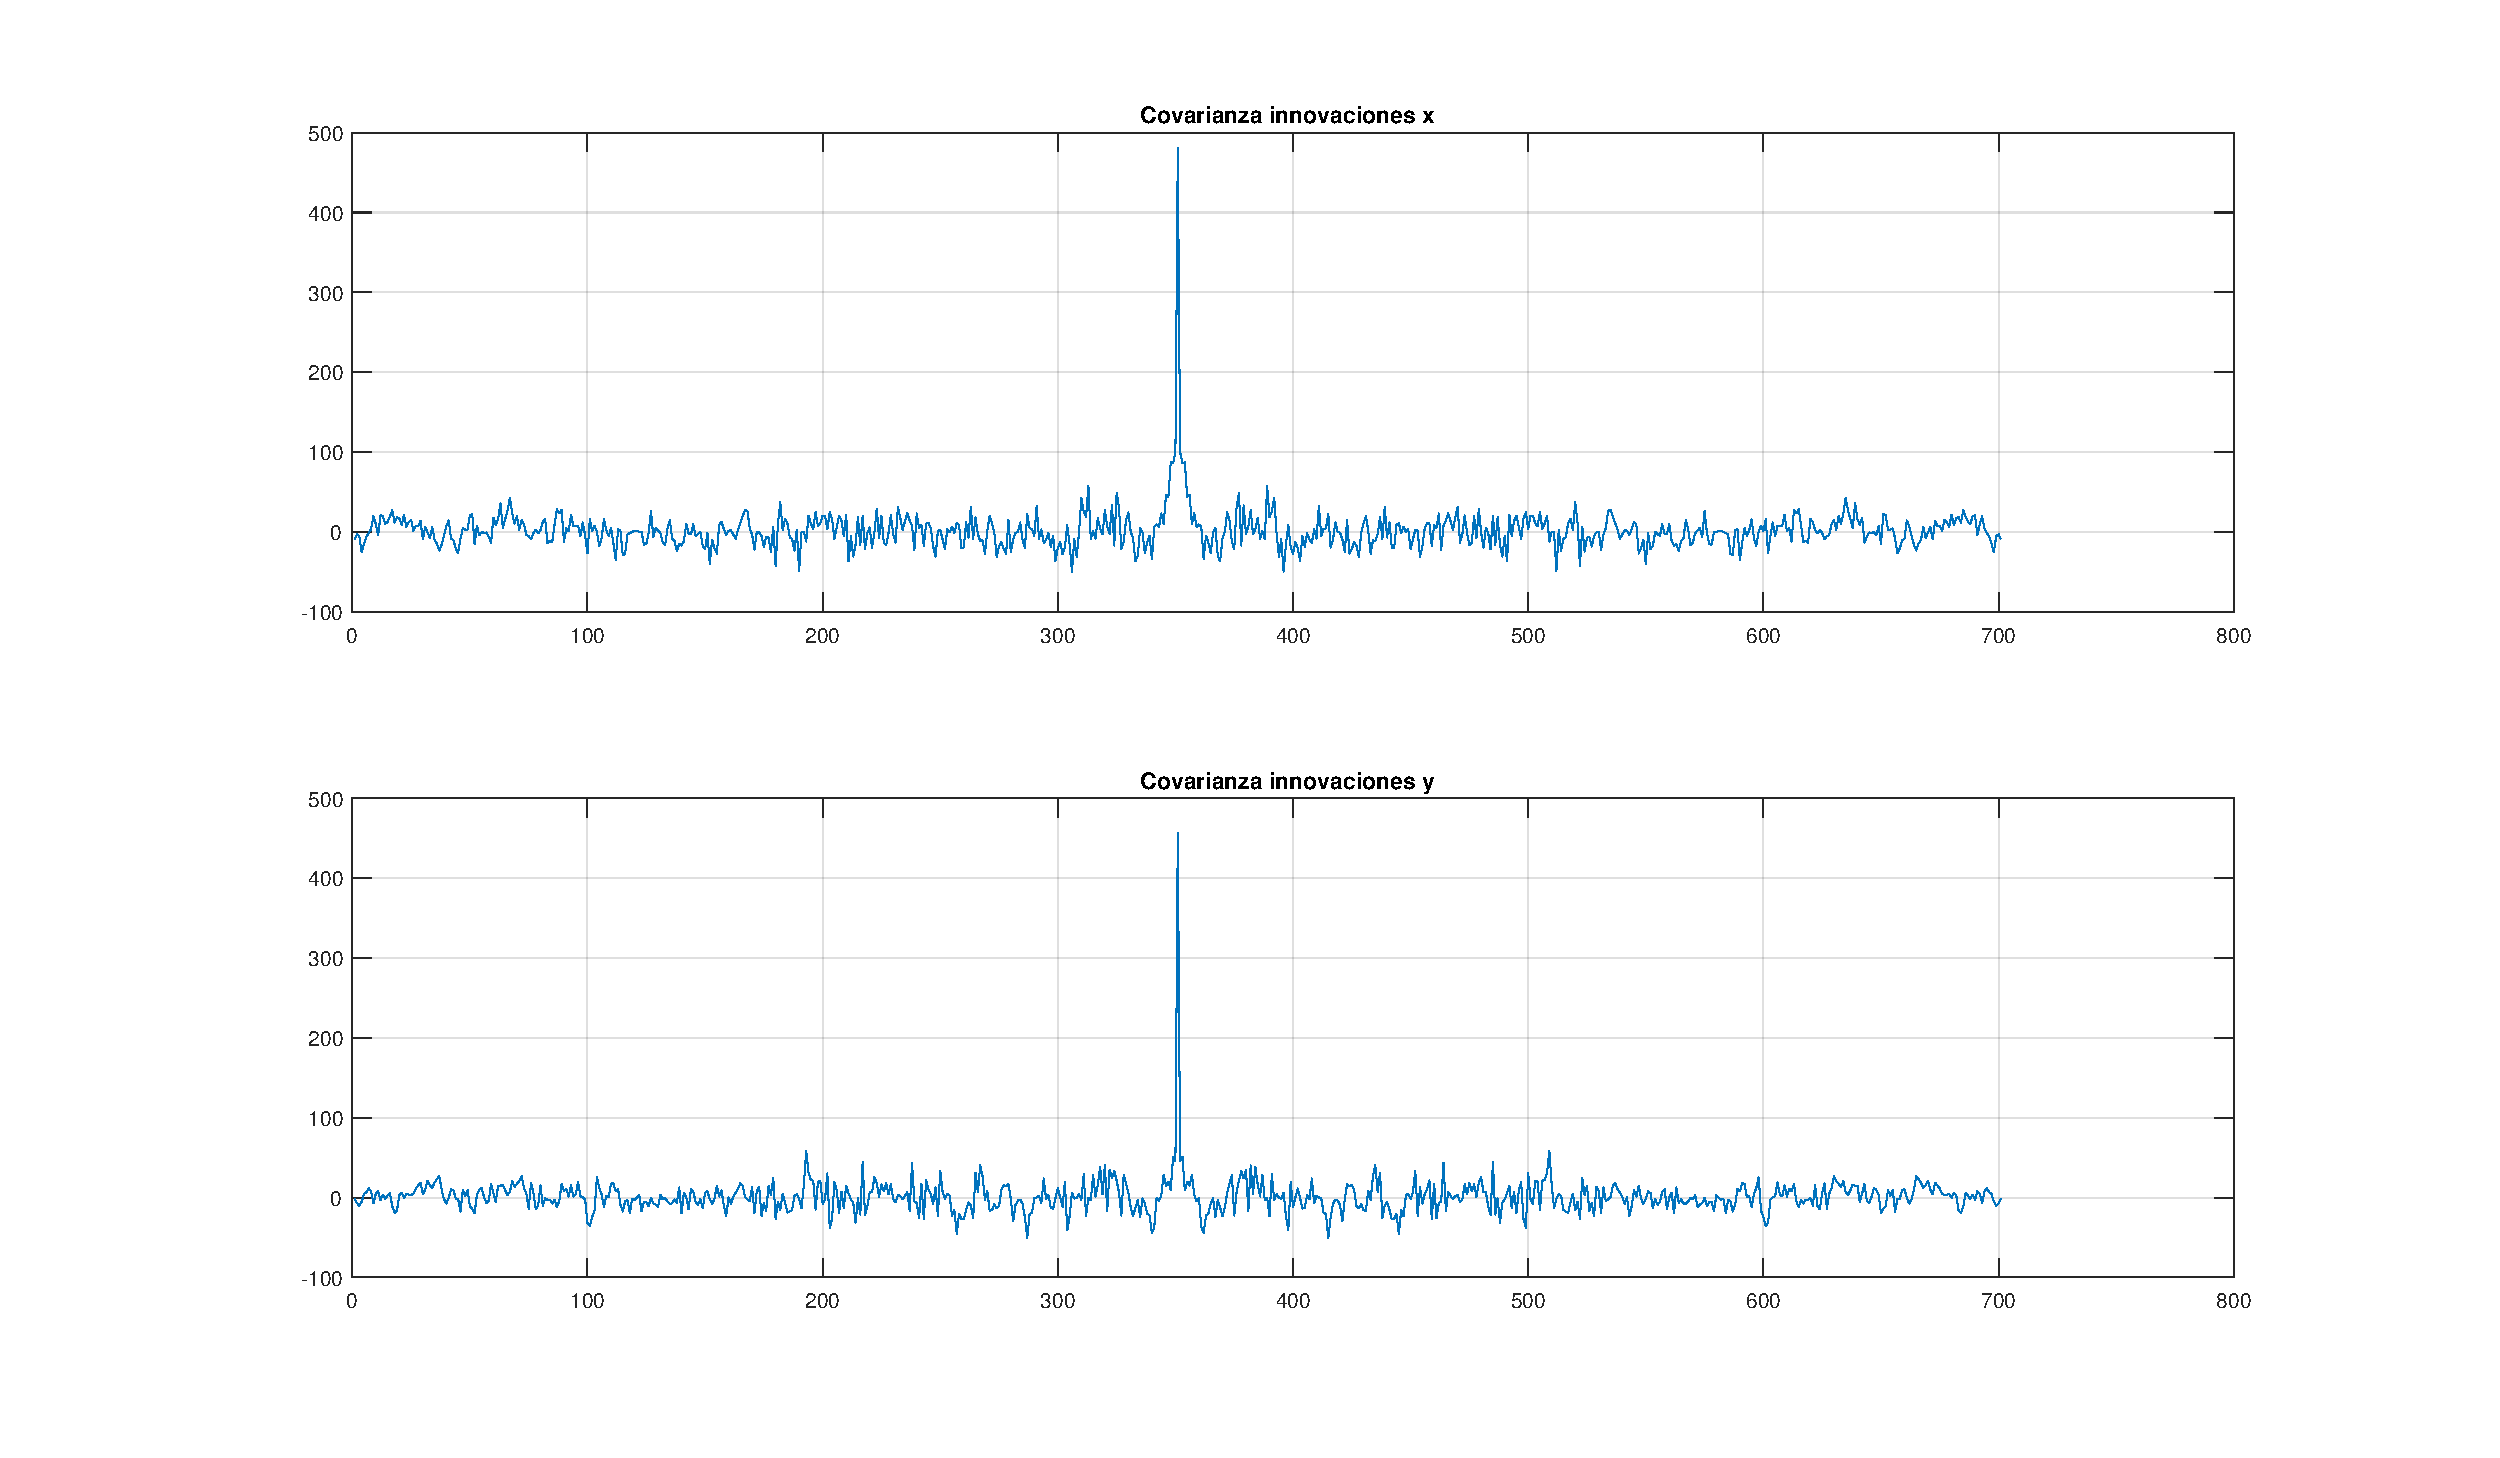
\includegraphics[width=1.0\textwidth,keepaspectratio]{Figuras/covinn_ej2c.pdf}
			\caption{Medición De Aceleración - Innovaciones}
			\label{fig:ej2c_innov}
		\end{figure}

	\subsection{Test De Observabilidad}
		Para determinar cuántos estados no observables tiene el sistema se debe analizar el rango de la 
		\Juan{Si hay ganas y se acuerda alguno, podríamos explicar esto.. for extra points}
		matriz de observabilidad. A continuación se expone la porción de código que se encarga de ello:
		\lstinputlisting[firstline=204, firstnumber=204]{EJ2_full.m}

		Para los incisios del ejercicio \ref{sec:ej2} se obtiene la siguiente tabla.
		\begin{table}[h!]
			\centering
			\begin{tabular}{ccc}
				\toprule
				Medición	& Cantidad no observables	& Observables\\
				\midrule
				$\vect{p}$	& 0				& $\vect{p}$ $\vect{v}$ $\vect{a}$\\
				$\vect{v}$	& 2				& $\vect{v}$ $\vect{a}$ \\
				$\vect{a}$	& 4				& $\vect{a}$\\

				\bottomrule
			\end{tabular}
				\caption{Test de observabilidad para el ejercicio 2.}
				\label{tab:obs_ej2}
		\end{table}

		Visualmente se puede comprobar, a partir de la inspección de las Figuras \ref{fig:ej2a}, \ref{fig:ej2b} y \ref{fig:ej2c}, que los estados observables son aquellos cuya medición se encuentra disponible y las derivadas de dicho estado. Los estados cuya derivada es la medición (es decir que el estado medido es la derivada) no pueden ser estimados correctamente dado que no son observables.

	\subsection{Script}
	
	A continuación se presenta el script de \texttt{MATLAB} que implementa el algoritmo. Se puede seleccionar si se está midiendo posición, velocidad o aceleración, estableciendo las variables \texttt{bool\_p}, \texttt{bool\_v} o \texttt{bool\_a} en 1 o en 0 para indicar que se esta midiendo.\\
	\lstinputlisting[firstline=18, firstnumber=18, lastline=20]{EJ2_full.m}
	\lstinputlisting[firstline=53, firstnumber=53, lastline=110]{EJ2_full.m}
